\documentclass[%
    %draft,
    %submission,
    %compressed,
    final,
    %
    %technote,
    %internal,
    %submitted,
    %inpress,
    reprint,
    %
    %titlepage,
    notitlepage,
    %anonymous,
    narroweqnarray,
    inline,
    twoside,
    invited
    ]{ieee}

\usepackage[utf8]{inputenc}
\usepackage[spanish]{babel}
\usepackage{graphicx}
\usepackage{verbatim}
\usepackage{moreverb}
\usepackage{amsmath}
\usepackage{amsfonts}
\usepackage{amssymb}
\usepackage{fancybox}
\usepackage{float}
\usepackage{fancyvrb}
\usepackage{subfigure}

\newcommand{\latexiie}{\LaTeX2{\Large$_\varepsilon$}}

%\usepackage{ieeetsp}    % if you want the "trans. sig. pro." style
%\usepackage{ieeetc}    % if you want the "trans. comp." style
%\usepackage{ieeeimtc}    % if you want the IMTC conference style

% Use the `endfloat' package to move figures and tables to the end
% of the paper. Useful for `submission' mode.
%\usepackage {endfloat}

% Use the `times' package to use Helvetica and Times-Roman fonts
% instead of the standard Computer Modern fonts. Useful for the 
% IEEE Computer Society transactions.
%\usepackage{times}
% (Note: If you have the commercial package `mathtime,' (from 
% y&y (http://www.yandy.com), it is much better, but the `times' 
% package works too). So, if you have it...
%\usepackage {mathtime}

% for any plug-in code... insert it here. For example, the CDC style...
%\usepackage{ieeecdc}

\begin{document}

%----------------------------------------------------------------------
% Title Information, Abstract and Keywords
%----------------------------------------------------------------------
\title[Métodos de búsqueda no informados]{%
       Métodos de búsqueda no informados}

% format author this way for journal articles.
% MAKE SURE THERE ARE NO SPACES BEFORE A \member OR \authorinfo
% COMMAND (this also means `don't break the line before these
% commands).
\author[Castiglione, Karpovsky, Sturla]{Gonzalo V. Castiglione, Alan E. Karpovsky, Martín Sturla\\\textit{Estudiantes 
       Instituto Tecnológico de Buenos Aires (ITBA)}\\
\\\textbf{15 de Marzo de 2012}
}



\journal{Cátedra\ \ Sist.\ de\ Inteligencia\ Artificial,\ ITBA\ }
\titletext{-\ 15, MARZO\ 2012}
\ieeecopyright{\copyright\ 2012 ITBA}
\lognumber{}
\pubitemident{}
\loginfo{15 de Marzo, 2012.}
\firstpage{1}

\confplacedate{Buenos Aires, Argentina, 15 de Marzo, 2012}

\maketitle               

\begin{abstract} 
El presente informe busca analizar y comparar distintas estrategias de búsqueda no informadas sobre un problema en particular (Skyscraper puzzle) haciendo uso de un motor de inferencias.
\end{abstract}

\begin{keywords}
DFS, BFS, General Problem Solver, depth-first, breadth-first, search strategy
\end{keywords}

%----------------------------------------------------------------------
% SECTION I: Introduccion%----------------------------------------------------------------------
\section{Introducción}

\PARstart El juego \textit{Edificios} también conocido como \textit{Skyscraper puzzle} es una variante del conocido \textit{Sudoku} y consiste de una grilla cuadrada con números en su borde que representan las pistas sobre cuántos edificios se visualizan en esa dirección. El tablero, visto desde arriba, representa un espacio cubierto de edificios. Cada casillero debe ser completado con un dígito que va entre 1 y N, siendo N el tamaño de la grilla; haciendo que cada fila y cada columna contengan sólo una vez a cada dígito (como sucede en el Sudoku).

%\par En este puzzle, cada dígito puesto en la grilla podría ser visualizado como un edificio de %esa altura. Por ejemplo, si ingresamos un 5, estaríamos colocando un edificio de altura 5. Cada %uno de los numeros que están por fuera de la grilla revelan la cantidad de edificios que pueden %ser vistos al mirar la línea o columna en esa dirección. Cada edificio bloquea la visión de todo %edificio de menor altura que se encuentre detrás de él.

%----------------------------------------------------------------------
% SECTION II: Marco Teórico
%----------------------------------------------------------------------

\section{Estados del problema}

\subsection{Estado inicial}

\par El estado inicial del problema es un tablero que contiene sólo las pistas en sus bordes (no contiene ningún edificio en la grilla). Para que el problema tenga solución éste tablero debe ser válido; es decir que no cualquier combinación de pistas sobre la visibilidad de edificios en esa dirección conducirán a un problema resoluble.

\subsection{Estado final}

\par El estado final del problema es un tablero con todos los casilleros completos (lleno de edificios) que cumpla con las reglas del juego citadas anteriormente.

\section{Modelado del problema}

\par El tablero del juego se modeló mediante la creación de la clase Board; la misma contiene una variable privada de tipo matriz de enteros que representa a la grilla propiamente dicha. Si un casillero de dicha matriz  tiene un $0$, significa que  está vacío; si en cambio tiene un número $k \in [1,n]$ significa que hay situado un edificio con altura $k$.\\
\par Las pistas o restricciones del tablero (números en los bordes del mismo) se modelaron con un arreglo de cuatro vectores de enteros (TOP, BOTTOM, LEFT, RIGHT) que simplemente contienen la restricción en esa dirección.
Cabe destacar que en los estados únicamente se guarda el tablero; guardar las restricciones sería redundante. Ver \textbf{Figura 1} en la sección \textbf{Anexo B}.\\



\section{Reglas}

\par Dado un tablero de tamaño $n\times n$ podemos describir las reglas del problema en forma general como sigue:

\emph{Poner un edificio de altura $x$ en la posición $(i,j)$ del tablero, con $x \in [1, n]$.}

\par Por lo que, que dado un tablero de $n\times n$, el total de reglas está dado por $n \times {n \times n} = n^3$ ya que por cada fila y por cada columna, se tienen $n$ edificios distintos para colocar. 
\par Ejemplos de reglas:
\begin{itemize}
\item Poner un edificio de altura 1 en la posición $(0,0)$
\item Poner un edificio de altura 4 en la posición $(3,1)$
\item $\ldots$

\end{itemize}

\par Las reglas así definidas producen un factor de ramificación de $n^3$ lo que hace que, para tableros grandes (mayores a $5\times5$) se tarde un tiempo muy considerable (en el orden de las horas) en encontrar la solución. Para subsanar este inconveniente se puede plantear el problema enunciando con un conjunto de reglas distinto, descripto a continuación:\\

\emph{Poner un edificio de tamaño $x$ en el próximo lugar disponible de izquierda a derecha y de arriba hacia abajo, con $x \in [1, n]$.}\\

\par En un tablero de $n\times n$ el conjunto de reglas quedaría definido de la siguiente forma:\\

\begin{itemize}
\item Poner un edificio de altura 1 en el próximo lugar disponible de izquierda a derecha y de arriba hacia abajo.
\item $\vdots$
\item Poner un edificio de altura $n$ en el próximo lugar disponible de izquierda a derecha y de arriba hacia abajo.
\end{itemize}

\par Esto otorga un factor de ramificación igual a $n$ siendo este muy inferior al del caso anterior. \\
\par Se decidió implementar ambos conjuntos de reglas y los resultados fueron comparados en las tablas de la sección \textbf{Anexo A}.

\section{Costos}

\par Debido a la naturaleza del probema, la aplciacion de todas las reglas tiene el mismo costo y éste es unitario. Es decir que la transición de un estado X a un estado Y, en nuestro caso, siempre cuesta $1$.

\section{Algoritmos de búsqueda implementados}

\par Hemos implementado cuatro algoritmos de búsqueda no informada diferentes. Los mismos son: DFS, BFS, IDFS, HIDFS.

\section{Heurísticas}

\par La idea detrás de las heurísticas, en un  problema de satisfacción de restricciones como el discutido, no es hallar el camino óptimo a la solución ya que previamente se conoce su profundidad y  costo,  sino descartar caminos que no conducirán al algoritmo hacia la solución. Esto se logra, para un determinado nodo, asignándole el valor \textit{infinito} a la función $h(n)$ de los sucesores irresolubles de éste.\\

\subsection{Heurística 1}

\par Si una restricción indica el número $1$, esa fila o columna deberá comenzar con la altura maxima $(n)$. Además si la restricción opuesta es un $2$, se coloca $n-1$ al lado de este.

\subsection{Heurística 2}

\par Dado un tablero de dimensión $n$, si una restricción indica algún número distinto de $1$ , esa fila o columna trivialmente no podrá comenzar con $(n)$.
\par Si se considera el caso general, si una restricción indica algún número $a$ mayor o igual que $1$ , esa fila o columna deberá tener un edificio con la altura máxima $(n)$ a, al menos, $a$ casilleros de distancia. Esto es fácil de verificar: si 
el edificio de altura máxima está a una distancia de $k$, a lo sumo puede haber $k$ edificios observados. Considerando que ambos lados tienen restricciones (izquierda y derecha ó arriba y abajo), se puede localizar a algunos casilleros donde está la altura máxima. Por ejemplo, si tenemos $K$ como restricción izquierda y $R$ como restricción derecha, esto implica que la altura máxima tiene que estar a, al menos, $R$ casilleros desde la izquierda y a, al menos, $K$ casilleros desde la derecha.
\par Pero aún se puede generalizar más. Sea $k$ la altura de un cierto edificio. Dado una restricción $a$, se verifica que el edificio de altura $k$ debe estar como mínimo a una distancia de $a - n + k$. La demostración es análoga a la anterior. Desde ya, si dicha distancia es menor o igual que uno no hay ningún 
tipo de información útil. Asimismo, cuanto mayor sea este número mayor es la información obtenida: las posibilidades para colocar el edificio con altura $k$ son menores. 
Es fácil ver que $ a + k - (n + 1) $ es la cantidad de casilleros que no pueden contener al edificio de altura $k$, por lo que se aplicará esta heurística únicamente cuando $ a + k - 1 > n$, es decir cuando el número en la restricción y 
la altura del edificio es relativamente alta comparado a $n$. 
\par De esta generalidad se obtiene un resultado útil. Dado una fila o columna con restricción $n$, cada edificio de altura $k$ debe estar al menos $n - n + k = k$ distancia. En otras palabras, el edificio de altura máxima debe estar a $n$ casilleros de distancia, 
el de altura $n-1$ a distancia $n-1$ o mayor, y así sucesivamente. Esto implica que los edificios deben estar ordenados de menor a mayor si se da esta situación.
\section{Resultados}

\par A través de las distintas pruebas realizadas se observó que el algoritmo con mejor desempeño cualquiera sea la dimensión del tablero, es el DFS. Ver tablas en la sección \textbf{Anexo A}. A su vez, entendiendo que para este trabajo los métodos debían ser desinformados y no podíamos aplicar heurísticas,  resultó interesante comparar los tiempos obtenidos en el punto anterior con los tiempos obtenidos dándole un órden particular a las reglas antes de que el \textit{General Problem Solver} comience a resolver. Básicamente lo que se hizo fue preprocesar las pistas o restricciones del tablero y ordenar el conjunto de reglas por única vez. Los tiempos obtenidos preprocesando las reglas fueron superiores a los anteriores pero aún muy inferiores al obtenido por el conjunto reducido de reglas.

\par Observando las tablas se puede apreciar que el algoritmo con mayor performance fue el DFS.

\section{Conclusión}

\PARstart Es notable destacar la cantidad tiempo requerido y uso de recursos para resolver pequeños problemas con métodos no informados. Luego de ver los resultados obtenidos para pequeños tableros, se necesitó hacer uso de un pre-ordenamiento de las reglas ya que la resolucion del problema tomaba un tiempo en el orden de las horas para tableros tan simples como ser $4\times4$.\\

\par Resultó muy interesante tambén la forma de resolver problemas mediante la aplicación del mismo conjunto reglas en forma repetida y variando el orden en cual se agregan los nuevos estados al conjunto de no explorados.

\par No sorprende que el DFS haya sido el algoritmo con mejor desempeño, dado que al tener un árbol con profundidad acotada, el DFS evita los inconvenientes más usuales como pasarse de la profundidad de la solución óptima o entrar en ciclos del grafo (la cota de profundidad le es muy útil). El IDFS tiene una performace menor dado que como el problema tiene profundidad acotada de $n$, el IDFS no es más que un DFS con el overhead extra de tener que iterar por las $n-1$ profundidades anteriores. El BFS resultó ser menos óptimo dado que son demasiados los estados que debe explorar para llegar a la solución en problemas exponenciales como es el de los \textit{Skycrapers}. 

%----------------------------------------------------------------------
% The bibliography. This bibliography was generated using the following
% two lines:
%\bibliographystyle{IEEEbib}
%\bibliography{ieeecls}
% where, the contents of the ieeecls.bib file was:
%
%@book{lamport,
%        AUTHOR = "Leslie Lamport",
%         TITLE = "A Document Preparation System: {\LaTeX} User's Guide
%                  and Reference Manual",
%       EDITION = "Second",
%     PUBLISHER = "Addison-Wesley",
%       ADDRESS = "Reading, MA",
%          YEAR = 1994,
%          NOTE = "Be sure to get the updated version for \LaTeX2e!"
%}
%
%@book{goossens,
%        AUTHOR = "Michel Goossens and Frank Mittelbach and
%                  Alexander Samarin",
%         TITLE = "The {\LaTeX} Companion",
%     PUBLISHER = "Addison-Wesley",
%       ADDRESS = "Reading, MA",
%          YEAR = 1994,
%}
%
% The ieeecls.bbl file was manually included here to make the distribution
% of this paper easier. You need not do it for your own papers.

%\clearpage

%\begin{thebibliography}{1}

%\bibitem{lamport1}
%Fierens, P. (2011),
%\newblock {\em Cuadrados mínimos: repaso},
%\newblock Buenos Aires: Instituto Tecnológico de Buenos Aires.

%\bibitem{lamport1}
%Abdi, H.,
%\newblock {\em  Least-squares: {Encyclopedia for research methods for the social sciences}},
%\newblock Thousand Oaks (CA): Sage. pp, 2003.

%\bibitem{lamport1}
%Farebrother, R.W. (1988),
%\newblock {\em Linear Least Squares Computations, STATISTICS: Textbooks and Monographs}, %\newblock New York: Marcel Dekker.

%\bibitem{lamport1}
%Lipson, M.; Lipschutz, S. (2001),
%\newblock {\em Schaum's outline of theory and problems of linear algebra}, 
%newblock New York: McGraw-Hill, pp. 69–80.


%\end{thebibliography}

%----------------------------------------------------------------------


\clearpage


\onecolumn
\section*{Anexo A: Tablas}

\textit{Nota: \textbf{N/A} significa que el algoritmo no encontró la respuesta en un tiempo razonable. Algunos tableros han sido corridos durante horas y otros durante varios minutos.}

\subsection{DFS}

\begin{table}[H]
\begin{center}
\begin{tabular}{|c|c|c|}
\hline
 & Conj. reglas 1 &  Conj. reglas 2\\
 & (estándar) &  (reducido)\\

\hline
\hline

&&\\
Tablero 1 & & \\
$(3\times 3)$ & & \\
&&\\
\hline
Tiempo & 245ms & 3ms \\
\hline
Nodos frontera & 82 & 4 \\
\hline
Nodos expandidos & 993 & 10 \\
\hline
Estados generados & 1076 & 15 \\
\hline
Profundidad de la solución & 9 & 9 \\
\hline
&&\\

\hline
\hline

&&\\
Tablero 2 & & \\
$(4\times 4)$ & & \\
&&\\
\hline
Tiempo & \textit{N/A} & 9ms \\
\hline
Nodos frontera & 290 & 3 \\
\hline
Nodos expandidos & 91236 & 93 \\
\hline
Estados generados & 91527 & 97 \\
\hline
Profundidad de la solución & 11 (cantidad edificios  & 16 \\
&puestos al corte)&\\
\hline
&&\\

\hline
\hline

&&\\
Tablero 3 & & \\
$(5\times 5)$ & & \\
&&\\
\hline
Tiempo & \textit{N/A} & 331ms \\
\hline
Nodos frontera & 935 & 7 \\
\hline
Nodos expandidos & 65729 & 901 \\
\hline
Estados generados & 66665 & 909 \\
\hline
Profundidad de la solución & 17 (cantidad edificios  & 25 \\
&puestos al corte)&\\

\hline  
\end{tabular}
\end{center}
\caption{Comparación de tiempos para DFS con distintos sets de reglas}\label{tablaIDFS}
\end{table}

\clearpage

\subsection{BFS}

\begin{table}[H]
\begin{center}
\begin{tabular}{|c|c|c|}
\hline
 & Conj. reglas 1 &  Conj. reglas 2\\
 & (estándar) &  (reducido)\\

\hline
\hline

&&\\
Tablero 1 & & \\
$(3\times 3)$ & & \\
&&\\
\hline
Tiempo & 3 sec 793 ms & 11ms \\
\hline
Nodos frontera & 0 & 0 \\
\hline
Nodos expandidos & 7132 & 16 \\
\hline
Estados generados & 7133  & 17 \\
\hline
Profundidad de la solución & 9 & 9 \\
\hline
&&\\

\hline
\hline

&&\\
Tablero 2 & & \\
$(4\times 4)$ & & \\
&&\\
\hline
Tiempo & \textit{N/A} & 58ms \\
\hline
Nodos frontera & 52836 & 1 \\
\hline
Nodos expandidos & 4132 & 111 \\
\hline
Estados generados & 57522 & 113 \\
\hline
Profundidad de la solución & 3 (cantidad edificios  & 16 \\
&puestos al corte)&\\
\hline
&&\\

\hline
\hline

&&\\
Tablero 3 & & \\
$(5\times 5)$ & & \\
&&\\
\hline
Tiempo & \textit{N/A} & 519ms \\
\hline
Nodos frontera & 152016 & 0 \\
\hline
Nodos expandidos & 3488 & 1889 \\
\hline
Estados generados & 155505 & 1890 \\
\hline
Profundidad de la solución & 2 (cantidad edificios  & 25 \\
&puestos al corte)&\\

\hline  
\end{tabular}
\end{center}
\caption{Comparación de tiempos para BFS con distintos sets de reglas}\
\end{table}


\clearpage

\subsection{IDFS}

\begin{table}[H]
\begin{center}
\begin{tabular}{|c|c|c|}
\hline
 & Conj. reglas 1 &  Conj. reglas 2\\
 & (estándar) &  (reducido)\\

\hline
\hline

&&\\
Tablero 1 & & \\
$(3\times 3)$ & & \\
&&\\
\hline
Tiempo & 802ms & 21ms \\
\hline
Nodos frontera & 82 & 4 \\
\hline
Nodos expandidos & 2583 & 57 \\
\hline
Estados generados & 2666 & 62 \\
\hline
Profundidad de la solución & 9 & 9 \\
\hline
&&\\

\hline
\hline

&&\\
Tablero 2 & & \\
$(4\times 4)$ & & \\
&&\\
\hline
Tiempo & \textit{N/A} & 68ms \\
\hline
Nodos frontera & 297 & 3 \\
\hline
Nodos expandidos & 28979 & 833 \\
\hline
Estados generados & 29777 & 837 \\
\hline
Profundidad de la solución & 10 (cantidad edificios  & 16 \\
&puestos al corte)&\\
\hline
&&\\

\hline
\hline

&&\\
Tablero 3 & & \\
$(5\times 5)$ & & \\
&&\\
\hline
Tiempo & \textit{N/A} & 1sec 643ms \\
\hline
Nodos frontera & 954 & 7 \\
\hline
Nodos expandidos & 25571 & 6528 \\
\hline
Estados generados & 26526 & 6536 \\
\hline
Profundidad de la solución & 19 (cantidad edificios  & 25 \\
&puestos al corte)&\\

\hline  
\end{tabular}
\end{center}
\caption{Comparación de tiempos para IDFS con distintos sets de reglas}\label{tablaIDFS}
\end{table}

\clearpage

\section*{Anexo B: Imágenes}

\begin{figure}[H]
\begin{center}
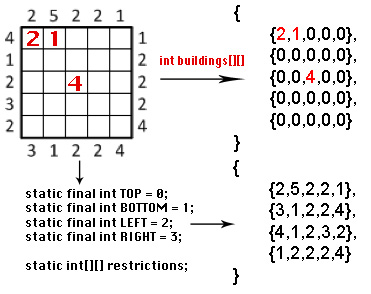
\includegraphics[scale=0.65]{./images/ModeladoSIA.jpg}
\label{modelado}
\end{center}
\end{figure}

\begin{center}
\par Figura 1: Modelado del problema
\end{center}


%\VerbatimInput{./code/calculoAb.m}




\end{document}